\section{新策略的独立配对验证与收益来源}
\label{field:sec-results}
\subsection{冻结规则、样本分工和实验分母}
实测日志用于识别移动占比高、重复无信号和清除接入等瓶颈，不作为可随意查询的世界。开发阶段仅使用6100000至6100149的150个合成世界/问，Q3七个、Q4八个有限配置共\FieldDevelopmentRuns{}次运行；比较原地补测、Q3负约束、路线组合、首项半径权重及安全清除接近。只增加补测、硬限制补扫次数或轻微缩环均不足以解释主要收益；最终保留原compact25和两题0.22固定探测比例，不将此前临时参数试探当作正式改进。

冻结后使用7100000至7100999的每问1000个新世界。Q3对照、仅路线、路线与信息、完整field四配置，Q4对照和field两配置，共6000次；三种压力位置、三种误差场、两策略、两题各50对（7200000至7200049），共1800次；随机位置的另两种误差各200对（7210000至7210199），共1600次。合计\FieldRuns{}次本地运行，全部完成全清并逐动作独立核对微秒计时。它们与20轮官方演练、早期10700次研究和2250次开发分别计数，不能相加称为独立世界数。

统计以每世界的$T_j/K_j$为等权单位，并按同一世界作差$d_j=T_j^{\rm refined}/K_j-T_j^{\rm field}/K_j$。配对均值差的近似95\%区间为$\bar d\pm1.96s_d/\sqrt n$。这说明合成分布下的均值不确定性，不是未来官方成绩的置信区间。参数、骨架与策略在本次确认前冻结，确认结果不再用于回调参数。

\subsection{相对已演练refined的直接比较}
\begin{table}[H]\centering\small
\caption{每问1000个新合成世界的配对结果，单位秒/源；不是官方反事实成绩}
\label{field:tab-main}
\begin{tabular}{lrrrrr}
\toprule
问题 & 策略 & 均值 & $p_{90}$ & 最坏 & 全清 \\
\midrule
Q3 & 原refined & 258.99 & 305.38 & 370.28 & 1000/1000 \\
Q3 & 仅路线改进 & 254.07 & 301.86 & 352.51 & 1000/1000 \\
Q3 & 路线与信息 & 251.13 & 299.49 & 340.73 & 1000/1000 \\
Q3 & 新field & 250.17 & 298.55 & 338.79 & 1000/1000 \\
Q4 & 原refined & 542.41 & 682.86 & 825.03 & 1000/1000 \\
Q4 & 新field & 508.60 & 642.48 & 760.05 & 1000/1000 \\
\bottomrule
\end{tabular}

\end{table}
问题三从\FieldQThreeControl{}降至\FieldQThreeTime{}秒/源，降低\FieldQThreeGain\%；问题四从\FieldQFourControl{}降至\FieldQFourTime{}秒/源，降低\FieldQFourGain\%。节省均值分别为\FieldQThreeSaved{}和\FieldQFourSaved{}秒/源，近似95\%区间分别为$[\FieldQThreeLower,\FieldQThreeUpper]$与$[\FieldQFourLower,\FieldQFourUpper]$；分别\FieldQThreeFaster/1000和\FieldQFourFaster/1000局更快。两题均1000/1000全清，不以降低清除率换时间。问题四$p_{90}$由682.86降至642.48秒/源，样本最坏值由825.03降至760.05秒/源。

\begin{figure}[htbp]\centering
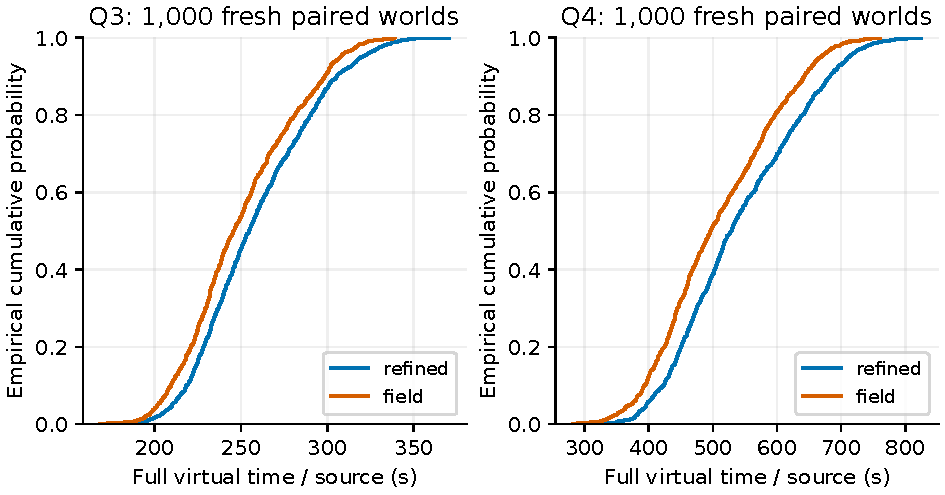
\includegraphics[width=\textwidth]{figures/field_performance.pdf}
\caption{已冻结field与原refined的同世界耗时分布；两题均保留原覆盖骨架与完整停止证书。}
\end{figure}

\subsection{消融和完整成本分解}
\begin{table}[H]\centering\small
\caption{相邻配置的配对节省，单位秒/源；信息项合并原地补测与Q3负约束}
\begin{tabular}{lrrr}
\toprule
问题 & 相邻配置 & 节省均值 & 近似95\%区间 \\
\midrule
Q3 & 原refined至仅路线改进 & 4.92 & [4.13, 5.70] \\
Q3 & 仅路线改进至路线与信息 & 2.94 & [2.59, 3.28] \\
Q3 & 路线与信息至新field & 0.96 & [0.87, 1.05] \\
Q4 & 原refined至新field & 33.81 & [31.61, 36.01] \\
\bottomrule
\end{tabular}

\end{table}
问题三的路线改进节省4.92秒/源，加入原地信息与负约束再节省2.94秒/源，安全接近再节省0.96秒/源。三者沿同一配置链比较，增量有条件性，不声称各机制脱离其他条件仍有相同贡献。问题四的主要收益来自路线组合；安全清除点移动在开发中没有体现稳定增益，因此对Q4关闭，不为堆叠机制而采用。

\begin{table}[H]\centering\small
\caption{按每世界每源的完整计费分解；移动含逐步微秒舍入，展示保留两位小数}
\begin{tabular}{lrrrrrrr}
\toprule
问题 & 策略 & 移动 & 检测 & 换频 & 失败清除 & 成功清除 & 合计 \\
\midrule
Q3 & 原refined & 195.50 & 48.98 & 9.32 & 0.19 & 5.00 & 258.99 \\
Q3 & 新field & 188.36 & 47.58 & 9.06 & 0.17 & 5.00 & 250.17 \\
Q4 & 原refined & 383.47 & 129.62 & 23.91 & 0.41 & 5.00 & 542.41 \\
Q4 & 新field & 350.93 & 128.53 & 23.66 & 0.48 & 5.00 & 508.60 \\
\bottomrule
\end{tabular}

\end{table}
Q3平均行程由12607.63降至12143.48米，Q4由24581.18降至22499.71米。Q4失败清除尝试均值却由1.782增至2.089次/局，说明不能把失败次数本身当作任务目标；它的增加被移动节省抵消。这里的失败统计是尝试次数/局，不是失败案例比例，所有案例最终均全清。

\subsection{压力、数值与现实运行边界}
22个压力或替代误差组全部全清，完整逐组均值、区间和更快案例数保存在\path{results/field_confirmation.json}及\path{report/generated/field_stress.tex}。Q4最小接收半径三组平均改善约5.90\%至7.06\%，边界向外三组约5.49\%至5.86\%；聚集平滑误差组的节省区间为$[-9.37,44.84]$秒/源，包含零，不能宣称在该组证实改善。Q3边界源收益较小，聚集组约0.53\%至0.63\%，不主张逐场景等比例下降，更不主张每局占优。

独立检查包含3000次负约束真实源包含性、1000米边界与退化域、双精度溢出拒绝、开放路线任务守恒、两任务可解析最优例、200组清除圆交接近及现实截止。保守内接多边形和顶点复验提供几何依据，随机检查只补充实现证据。两题新策略在主检验中本地单局最大运算耗时分别约\FieldQThreeWall{}秒、\FieldQFourWall{}秒；这些数值不包含官方HTTP延迟，不能替代20分钟现实期限的实测。现有20轮官方日志验证的是原refined，新field必须在新的官方演练局确认，正式测试仍需各题三次原始结果及加密日志。
